
% Materials and Methods
%6. Summary of Publication Recommendations
%Published reports must contain sufficient detail to allow other
%experimenters to try to replicate the reported results and to help
%explain failures of replication. Given the limited space that journals
%provide, recommendations will be summarized below for both
%necessary and optional recording and environmental procedures to
%be reported in publications of studies using EDA.
%First and above all, the method of measurement has to be specified:
%endosomatic or exosomatic, direct or alternating current (if
%any) applied to the skin, and constant voltage or constant current.
%The applied voltage (or current) must be noted. If commercially
%available instrumentation has been used, the manufacturer and
%instrument type should be mentioned. Furthermore, calibration
%procedures should be specified.
%Second, methods of signal conditioning and storage need to be
%specified, including procedures for separating EDL from EDRs,
%if applied, time constants of amplifiers, separate grounding procedures,
%if used, A/D conversion rate, and sampling frequency
%(for EDL and EDRs if stored separately).
%Third, recording sites should be specified for active and inactive
%electrodes (if applicable). If the sites were pretreated, the procedure
%should be reported in detail. Also essential is providing details for
%electrodes and electrolytes that were used, such as electrode metal
%(e.g., sintered Ag/AgCl), area of contact (either in square centimeters
%or diameter), method of fixation (e.g., double-sided adhesive
%tape), details of the used electrolyte, such as type of gel or base,
%ionic type and concentration (e.g., 0.08 M or 0.5% NaCl), or, in the
%case of disposable electrodes, brand and type plus as much of the
%above mentioned information as is available from the manufacturer. It is important to know how long electrodes were attached
%before the recording started and how long they stayed in place.
%Details of how polarization was controlled and how electrodes
%were stored should be given if available. In the case of DC recording,
%we recommend using a polarity reversal switch between segments
%within a session.
%Fourth, signal evaluation needs to be reported in detail, whereas
%the sampling rate (for tonic and phasic measures separately, if
%different) and specification of time windows for tonic and phasic
%measures (e.g., latency windows for EDR onset being 1–4 s after
%stimulus onset) are mandatory. For EDRs, a minimum amplitude
%criterion must be specified and reported (e.g., 0.01 mS for SCRs to
%be scored). The standard terminology mentioned in Section 3
%should be adhered to. The term EDR magnitude should be reserved
%for the average amplitude calculated from a series of responses that
%include zero amplitudes. Any treatment of superimposed EDRs
%should be specified. Methods of detection and elimination of
%recording artifacts should be described if applicable.
%Besides the usual details to be reported about procedures for
%laboratory and field settings, it is important for EDA measurement
%to specify baseline conditions in detail, including length and statistical
%treatment during EDAdata evaluation. The gender, age, and
%ethnicity of the participants (e.g., number, range or mean, and
%standard deviation) are essential for comparison with EDA results
%from other studies. Medication or drug use (including caffeine
%intake before participation in the study) need to be reported as well.
%Clothing as well as inside and outside temperatures and their possible
%changes during the recording periods should be reported in as
%much detail as possible. If available (e.g., in case of room airconditioning),
%relative humidity should be reported as well.

\section{Materials}
% mention the SNNU and the lab where the study takes place
All experiments and measurements were conducted within the facilities of Systems Neuroscience and Neurotechnology Unit, especially the Green Lab, which is located at the Saarland University Hospital. 

\subsection{System Components}
%In this section all the components that are necessary to run the virtual reality system are described.
% It is to mention that the used parts were primarily selected in regard to their availability and the system as a whole was kept as cost-efficient as possible. The system can therefore be very appealing to a variety of users, in need of a low-budget treatment system, suited to be operated in limited spaces.
The virtual reality system is comprised of a number of components, some of which were created in the scope of a different thesis\footnote{This is a reference to the master thesis of Santhosh Nayak, a fellow student, contributing to the project.}. Therefore, this section will focus on components that were built in the scope of the present thesis and delineate what is necessary to run the virtual reality system.
  
\subsection{Hardware}\label{Hardware}
\subsubsection{HTC Vive}
The Vive is a commercial virtual reality system that has been developed by HTC in cooperation with Valve and is composed of a Head-Mounted Display (HMD), a tracking system, called Lighthouse, and two controllers. Inside the virtual environment, which is presented to the user via the HMD, the user's position is tracked by the Lighthouse-System at all times, allowing for the user to explore the virtual environment. The Tracking system is composed of a minimum of two base stations, which are located at the edge of the intended tracking area, approximately 2m above the ground. In addition the controllers can be used to perform tasks and to interact with objects inside the virtual world. The Vive can be used in combination with a any computer fitting the following minimum requirements. 
  
\textbf{System Requirements}
\begin{itemize}
\item Graphics: NVIDIA GeForce™ GTX 1060 or AMD Radeon™ RX 480, equal or higher
\item CPU: Intel™ Core™ i5-4590 or AMD FX™ 8350, equal or higher
\item RAM: minimum of 4 GB RAM
\item Video port: 1x HDMI 1.4-port or DisplayPort 1.2 or newer
\item USB ports: 1x USB 2.0-port or newer
\item Operating System: Windows™ 7 SP1, Windows™ 8.1 or newer or Windows™ 10
\end{itemize}

\textbf{Tracking Space Requirements}\\[10pt]
To guarantee a satisfying experience a minimum room size of 2m x 1.5m with a maximum distance of 5m between base stations is suggested by the manufacturer. 
% descibe calibration , room measurement, visible barrier ,Das Chaperone-System warnt Sie über die Grenzen Ihres Spielbereichs, sodass Sie in VR eingetaucht bleiben können, ohne sich über die reale Welt Gedanken zu machen. 
\subsubsection{BITalino}
The BITalino (r)evolution Plugged kit is an innovative low-cost toolkit that was developed for rapid prototyping of wearable devices and biomedical signal acquisition. The main board, or BITalino Core, is comprised of for major components, the Microcontroller (MCU) Block, the Bluetooth Block, the Power Block with the device's own LiPo battery and the UC-E6 connectors. The MCU features 12 ports, which are divided into 8 analog and 4 digital ports. Of the 7 separately included BITalino sensors, which are connected via cable, only the EDA sensor and the ECG sensor were used. The data is recorded with one of the 4 preset sampling rates and then sent to the user's computer, via a Bluetooth connection. The BITalino is supported by a number of platforms, such Matlab and Unity, allowing for easy implementation in almost any data acquisition process.\\

\begin{figure}[ht]
\centering
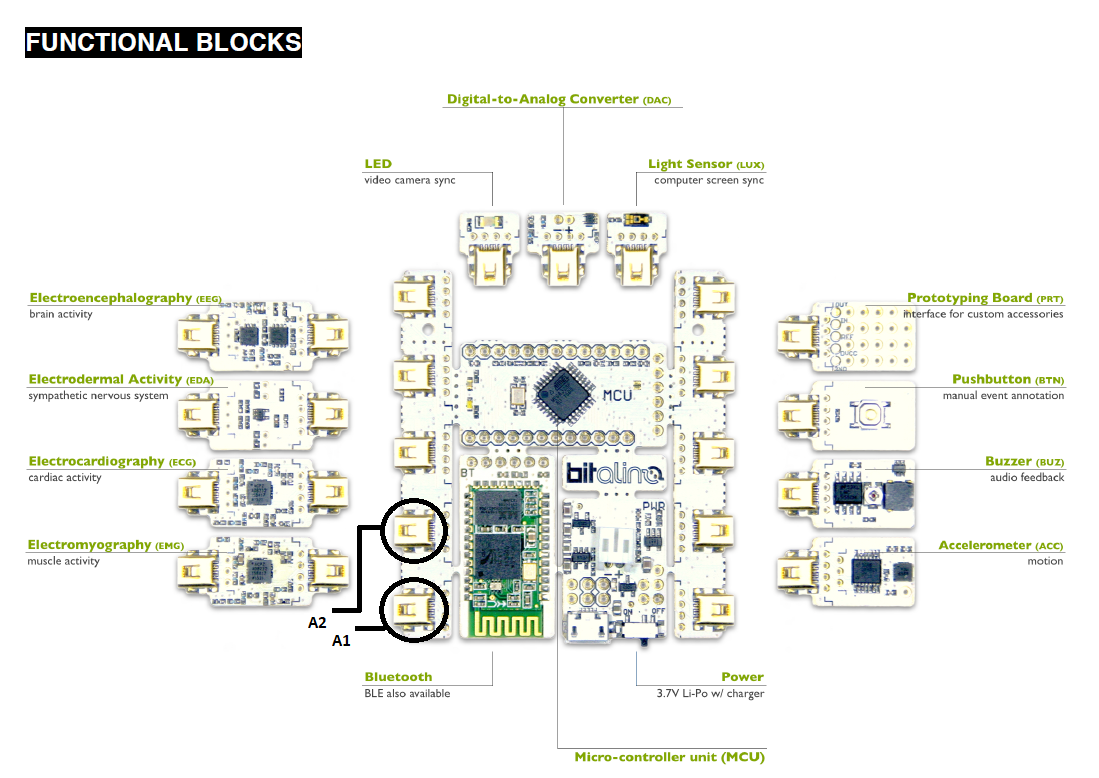
\includegraphics[width=0.7\textwidth]{images/BitOverview.png}
\caption{Graphical overview of the BITalino device including all functional blocks.}
\label{bitImg}
\end{figure}

\textbf{Specifications}
\begin{itemize}
\item Analog Ports: 4 in (10-bit) + 2 in (6-bit) + 1 auxiliary in (battery) + 1 out (8-bit)
\item Digital Ports: 2 in (1-bit) + 2 out (1-bit)
\item Sampling Rate: 1, 10, 100 or 1000Hz
\item Communication: Bluetooth
\item Sensors: ECG, EDA
\item Size: 100x65x6mm
\item Power Supply: LiPo battery (500mA, 3.7V)
\end{itemize}

\textbf{Accessories}
\begin{itemize}
\item 1x EDA Sensor
\item 1x ECG Sensor
\item 1x 3-lead cable
\item 1x 2-lead cable
\item 2x UC-E6 to UC-E6 sensor cable
\item pre-gelled electrodes
\end{itemize}

\subsubsection{VR Unit (VRU)}
VRU is the expression given to the computer, which is used to run the Unity software and power the HMD while the system is in use. It is to mention that the performance of the HTC Vive, in some degree, is reliant on the CPU and GPU of the VRU. Therefore exceeding the minimum requirements, although involving higher cost, has proven to beneficial for the user experience, especially when the used virtual environment relies on realistic real-time lighting effects. On a monitor, which is connected to the VRU, the virtual world, as perceived by the HMD, is displayed for the user to see. However, while the system is in use, the software that is run on the VRU is controlled by a separate computer. Therefore it is essential that the VRU is able to connect to the internet. Alternatively a local network can suffice given one of the following conditions is met:\\[10pt]
a) the CMU (see \ref{CMU}) is located in the same local network as the VRU\\
b) the functions of VRU and CMU are handled by a single computer\footnote{If this variant is used, a Bluetooth adapter is required to connect to the BITalino device.}\\[10pt]
 
\subsubsection{Control and Measurement Unit (CMU)}\label{CMU}
In the early design phase the CMU was conceptualized as a part of the VRU, but it was then separated in regard to its intended use as a mobile control device for the therapist during the therapy. However, in our experiment a Laptop served as CMU. The CMU enables the user to submit orders to the VRU, control the BITalino, as well as to view the preprocessed Data. To find detailed explanations to the functions mentioned above, see \ref{Methods}.

%\subsubsection*{Conclusion}
%In conclusion it can be said that the system at hand certainly is built to perform on a minimum budget but also be applicable to a number of clinical applications, particularly the treatment of phobias
\subsection{Software}
As mentioned in section \ref{CMU} the data acquisition is handled by a separate computer. However, all programs were designed to function on any device, capable of running the software in this section. 

\subsubsection{Unity}
Unity is a game development platform, which can be used to create high-quality 3D games and deploy them across a variety of platforms, mobile phones, tablets and desktop computers. The user is enabled to directly target a VR device through the implemented Unity VR Software Development Kits (SDK). The VR environment is built by creating game objects, such as structures and lights, and placing them inside a three dimensional virtual space or importing prefabricated assets from the Asset Store. Each game object can be equipped with a number of components to fit the user's needs. One of the most important aspects to the Unity platform is its scripting API that gives the user control over the game environment. This is accomplished by C\# scripts, which are created in Visual Studio 2017 and then attached to the  specific game objects. As a game development platform Unity naturally is provided with an extensive networking environment, including UDP and TCP/IP, which can be used for communication with external devices. In addition the support, offered to the user in form of the Unity Manual and Scripting API as well as the Asset Store, is sufficient to allow even non-professionals to create their own projects.

\subsubsection{Matlab}
Matlab is a software, which was created to solve mathematical problems. It is used for data acquisition and processing as well as feature extraction from the measured signals.

\subsection{Virtual Environment}
As mentioned earlier there are two major requirements that must be met to successfully treat phobias with virtual exposure, fear elicitation and emotional processing. To elicit fear in the subjects we have to ensure that adequate stimuli are offered in our virtual environment. We therefore have implemented three different ways to adapt the difficulty of our virtual height scenario. The virtual environment was designed around the concept of a descending floor inside a closed room. In the default configuration, which is shown in figure \ref{VRdefaultImg}, a neutral environment is provided.

\begin{figure}[ht]
\centering
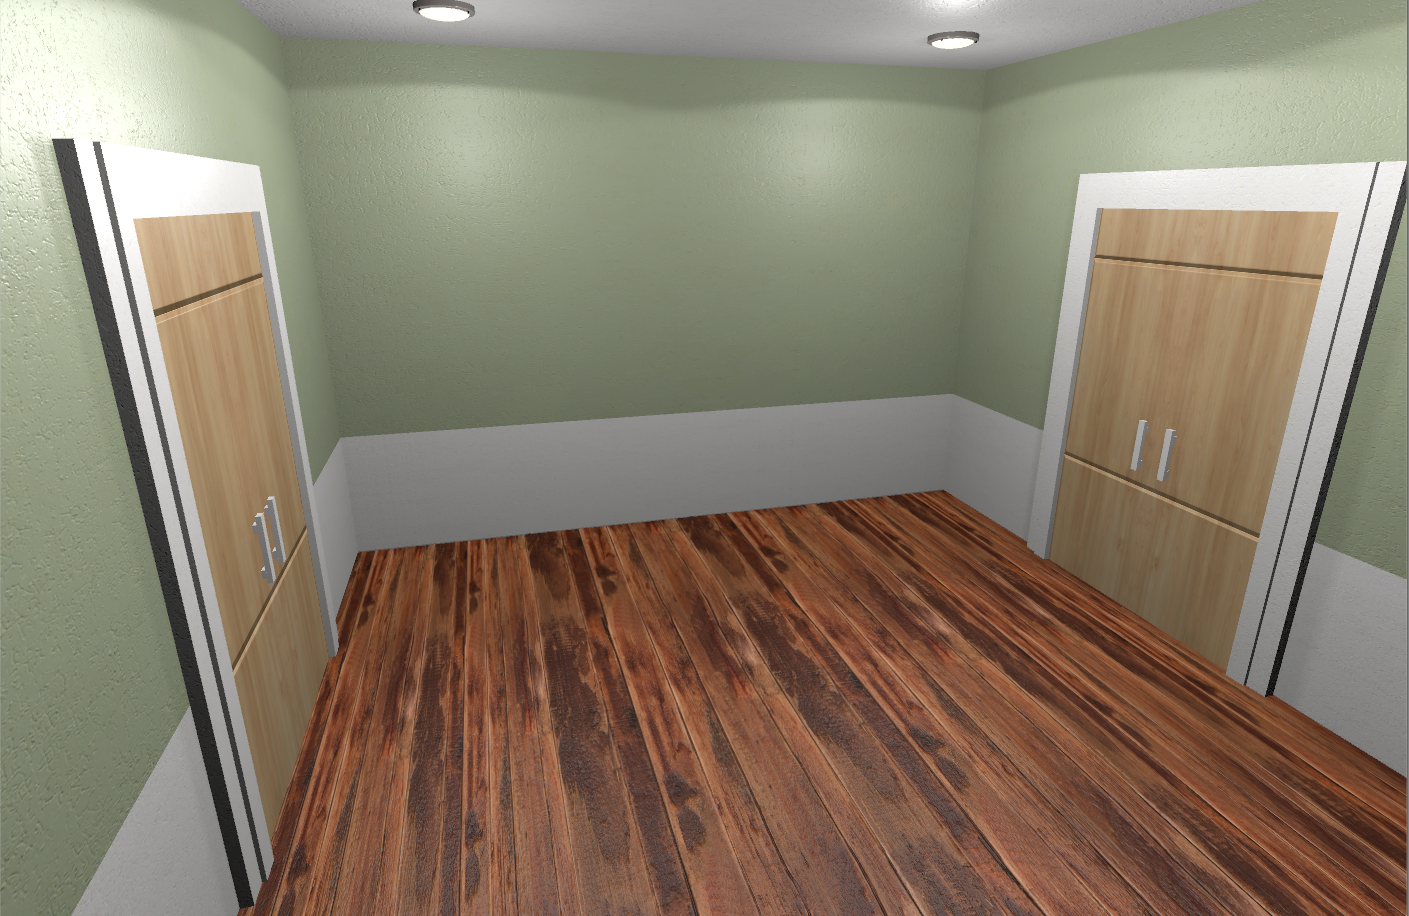
\includegraphics[width=0.7\textwidth]{images/RoomDefault.png}
\caption{A side view of the VR room in its default configuration.}
\label{VRdefaultImg}
\end{figure}

\begin{figure}[ht]
\centering
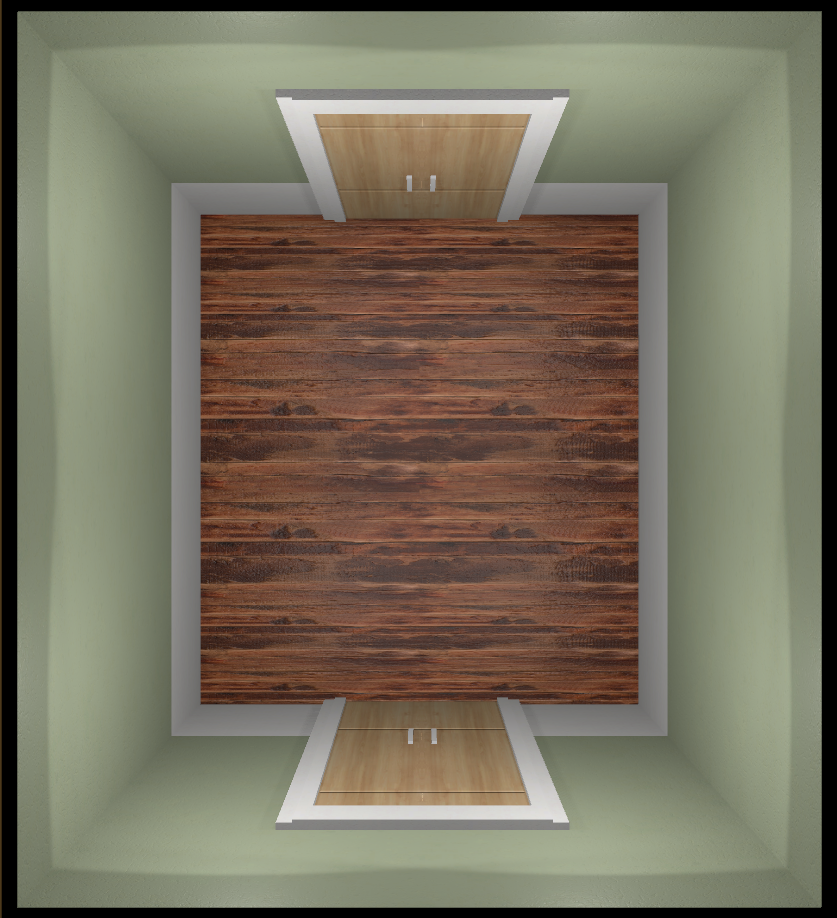
\includegraphics[width=0.7\textwidth]{images/RoomDefaultTop.png}
\caption{A top view of the VR room in its default configuration.}
\label{VRdefaultTopImg}
\end{figure}

This configuration is used at the start of the session to conduct baseline measures and to allow for acclimation to the virtual reality. The first stimulus that is presented to the patient is the opening of the floor, which is shown in figure \ref{OpenImg}. Initially the floor was programmed to open completely. This was later adapted in regard to a recommendation by the psychiatry department. It was suggested that the ability to gradually move the floor to the side and therefore provide a form of minimal stimulation could be particularly useful in the treatment of very severe cases of acrophobia. Thus, two additional steps were implemented at the one third and two third mark of the full opening distance.

\begin{figure}[ht]
\centering
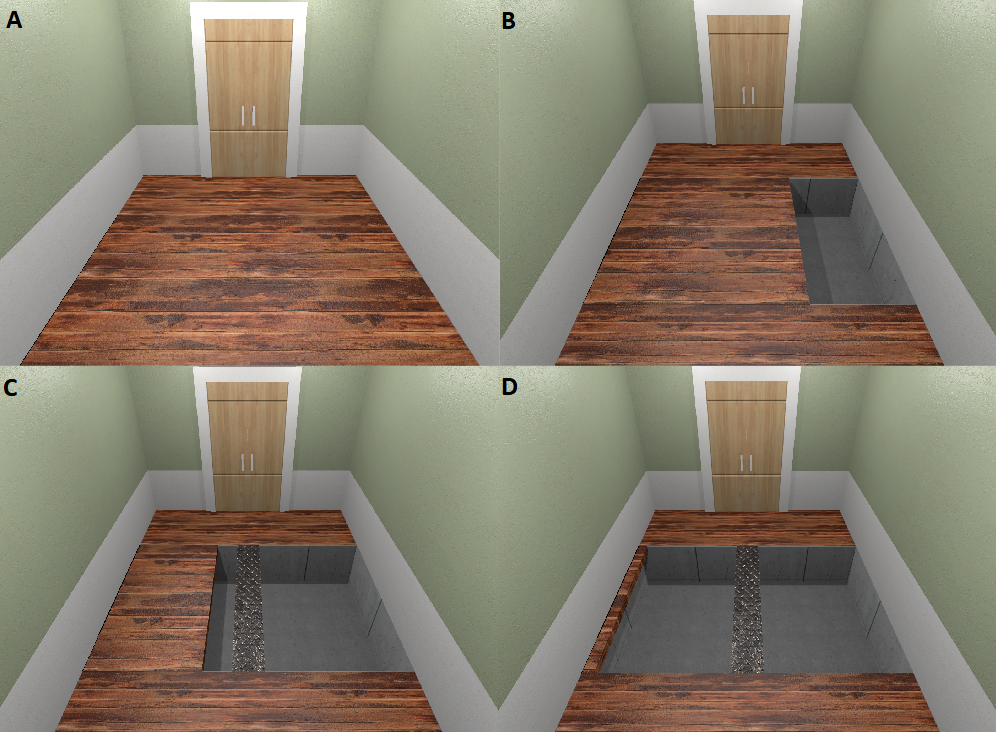
\includegraphics[width=0.7\textwidth]{images/OpenComparison.png}
\caption{Comparison of the different stages of floor opening.}
\label{OpenImg}
\end{figure}

The actual height challenge as well as the two remaining stimuli are revealed once the floor has been opened up. The patient is then confronted with a narrow bridge located above a descendable platform that is initially positioned 1m below floor-level (see \ref{OpenImg}, D). During therapy patients are asked to cross the bridge in order to confront their fear. A task, which in this state of the virtual environment, is considered to be of a lower difficulty. However, the difficulty can be adapted to each individual by alterations made to the strength of the primary stimulus, the depth. The platform can be lowered to a depth of up to 40m, enabling a degree of stimulation that could hardly be achieved in in-vivo exposure. But there are also precautions to be made to guarantee that the full extend of this stimulus can be perceived by the patients.
For instance there are no natural light-sources in a closed room scenario. Therefore the virtual room has to be equipped with an operant lighting system. We have applied 4 ceiling lamps that each are featured with 2 different light-sources, a point and a spotlight. Point lights are located at a certain point inside the virtual space and send out light, which is equally distributed, in all directions. The intensity of the eradiated light is diminished with increasing distance to the source, eventually reaching zero at the a specific range, which was set to 13m. We have used point lights to simulate the natural patterns of light in close proximity to a big surface lamp. The glow of the light bulb itself was recreated by using a material property called emission, causing light to be emitted directly from an object's surface to which the material has been applied. Spotlights too have a specified location and range but are used to illuminate a constrained angle, resulting in a cone shaped region of illumination. In addition to the previously mentioned range specific intensity drop off, the intensity of the spotlight is reduced from the inside to the outside of the light cone, causing a fade effect in the outskirts region, the so called penumbra. We have used spotlights with a range of 13m and an angle of 165 degrees to light the room as well as the initial section of the pit. As the platform is lowered beyond this range it is obscured by shadows and becomes less visible. Therefore we have implemented additional light-sources that are activated and deactivated according to the current platform position. Thus, the platform is sufficiently illuminated at all times (see \ref{DepthImg}, C and D).

\begin{figure}[ht]
\centering
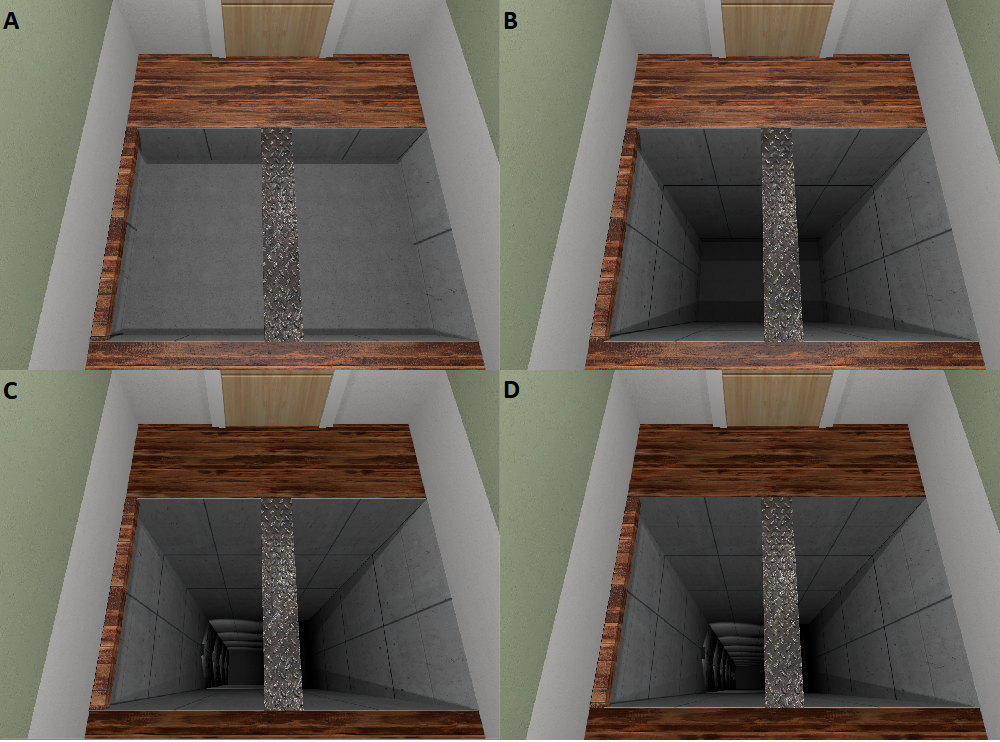
\includegraphics[width=0.7\textwidth]{images/DepthComparison.png}
\caption{Illustration of 4 different platform position.}
\label{DepthImg}
\end{figure}

In figure \ref{DepthImg} four different depths, subsidiary for four stimulus intensities, are displayed: A = 1m, B = 8m, C = 25m and D = 40m. It has to be mentioned that those depths only were chosen to illustrate different therapy difficulties whereas the depth can be freely changed in steps of 1m. Earlier we have talked about the immersion being disrupted by changing scenes during the session. To counter this phenomena, we have programmed the transition phase between difficulties to be smooth and gradually instead of the floor being abruptly teleported to the new target location. 
The third available method of increasing the difficulty is an alteration to the width of the bridge. This also was implemented after a suggestion of the psychiatrists involved, improving the adaptability of our system. Similar to the opening of the floor we have decided for a total of four different widths, ranging from 25cm to 1m (see \ref{BridgeImg}).

\begin{figure}[ht]
\centering
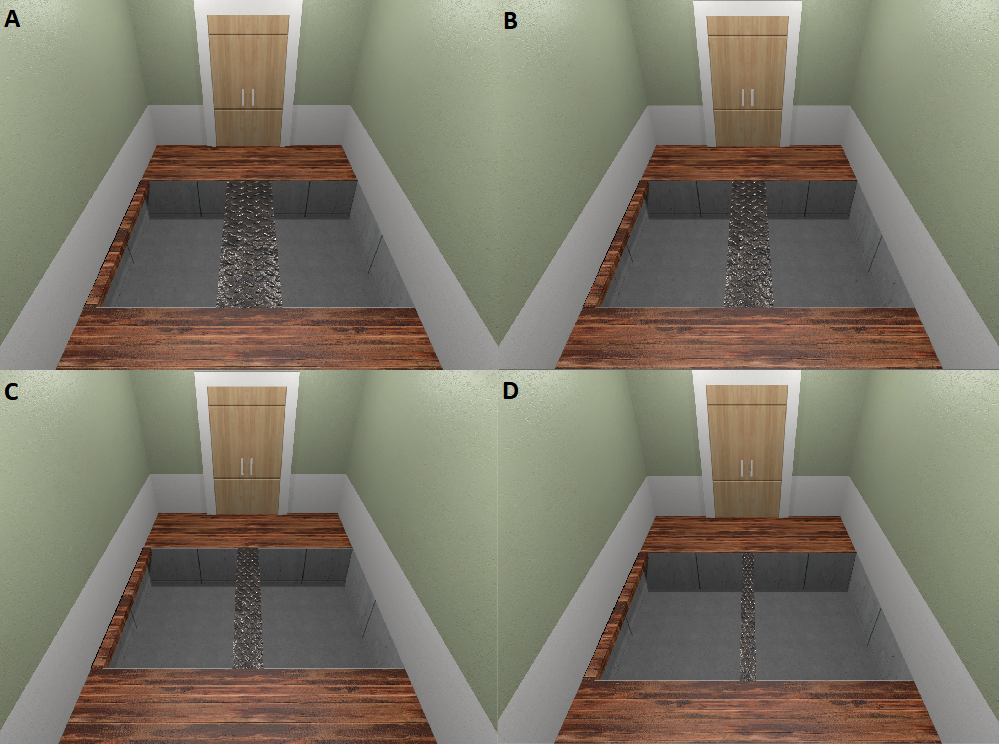
\includegraphics[width=0.7\textwidth]{images/BridgeComparison.png}
\caption{Comparison of the different widths of the bridge.}
\label{BridgeImg}
\end{figure}

As full control is given over these three variables the therapist is enabled to adjust the exposure a every degree of fear. 
The methods that were used to enable control of the virtual environment are explained in section \ref{VRControl}.

\subsection{Virtual Reality Setup}
To display the virtual environment, a powerful computer(Intel(R) Core(TM) i7-3770, 3.4 GHz and 8 GB RAM) and an Nvidia GeForce GTX 1080 graphics card with 8 GB of dedicated memory (GDDR5X) were used in combination with the HTC-Vive Head-Mounted Display (HMD). The Dual AMOLED displays (3.6" diagonal) of the HMD provided for a high-resolution presentation of the virtual world, with 1080x1200 pixel on each eye. The distance between the pupils was manually adjusted for each participant by means of a knob on the HMD to guarantee clear vision. 
% The Lighthouse Tracking-System, created by the company Valve, allowed to track participant's motion during the exposure in an area of maximal 5 by 5 meter and to project their movement in the virtual environment., and all the sensors, which were attached to the HMD and the controller by HTC. 
Two base stations of the Lighthouse system were positioned in opposing corners at a height of roughly 2 m. Due to limited space, the exposure area was restricted to an area of 3.5 by 3.5 meter. The program, which was used to remotely control the virtual environment, was written with the Matlab software version R2015a and run on a Laptop (Intel(R) Core(TM) i5 6200U, 2x2.3 GHz and 8 GB Ram). The virtual environment was run on the desktop computer, using Unity version 5.6.1f1 personal. Both machines were connected through a closed network. We have used the BITalino device to record the physiological data and send it to our Laptop via a Bluetooth connection. We have chosen this device primarily for the convenience of wireless data transmission, higher maneuverability and less distraction for the patient. 

\subsubsection{Closed Loop Information Flow}
The key concept of our system was the adaptability of the virtual experience to the therapist standards as well as the individual standard. To achieve our goal we built our system in a way that information is constantly exchanged between the single components.
The setup is composed of four major components that can be divided into two groups according to their function. Either the information is delivered to the subject (VRU and HMD) or retrieved from the subject and presented to the user (CMU and BITalino) (see figure \ref{setupImg}).\\ 

\begin{figure}[ht]
\centering
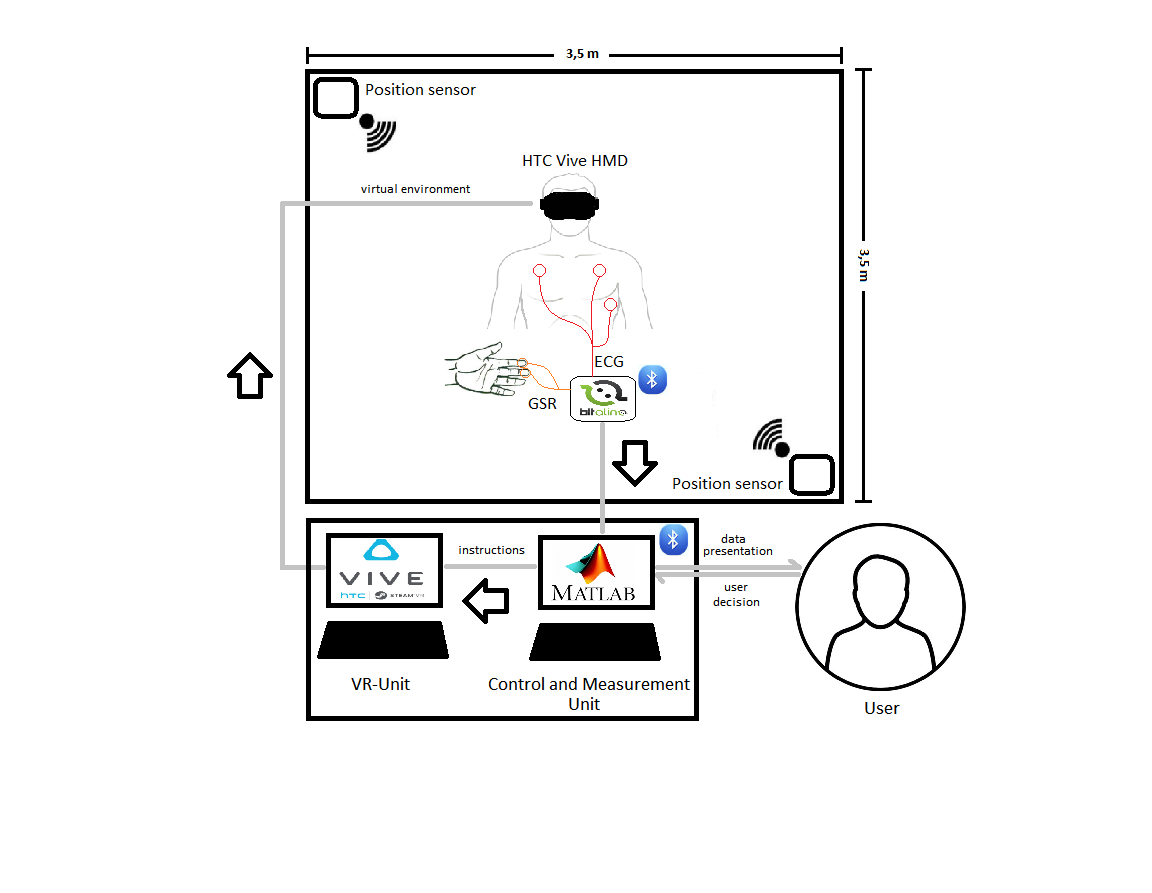
\includegraphics[width=0.9\textwidth]{images/setup.png}
\caption{Closed-loop virtual reality system. The grey line illustrates the closed loop information flow.}
\label{setupImg}
\end{figure}

The virtual environment was run on the VRU and presented to the subjects through the HMD. Inside the virtual environment the fear triggering stimulus was applied, causing a sympathetic reaction in the subject. This reaction was measured by the BITalino device, in the form of an ECG and GSR signal, and then sent to the control and measurement unit (CMU) via Bluetooth. Afterwards the data was processed by the CMU and displayed, in real-time, for the user to evaluate. Simultaneously the virtual world was displayed to a monitor, which allowed the user to see the perspective of the subject during the exposure. Based on the visual input, a decision to alter the virtual experience could be made by the user. This information was then submitted to the VRU, causing the virtual environment to react accordingly and therefore closing the information loop.


\newpage
\section{Methods}\label{Methods}
% methods
%- main objective is the measurement of gsr during the therapy and the evaluation of the gsr data concerning the stress of the patient during the therapy\\
%- how is the gsr information processed and evaluated?\\
%how is it presented to the user?\\
%- description of how the VR is controlled by the user(which parameters can be influenced)
%- graphic of control chain

\subsection{Participants}
\subsection{Procedure}
\subsubsection{Subject instruction}
Additionally the infrared connection between the base stations of the Lighthouse-System and the HMD should be kept intact at all time
\subsubsection{VR initialization}
%https://docs.unity3d.com/Manual/VROverview.html

\subsection{Virtual Reality Control}\label{VRControl}
One of the major challenges, we were confronted with during this project, was to find a method that would allow for a reliable information transport between VRU and CMU. We have decided on a TCP/IP solution for this problem. This allowed for a loss-free data transmission between the two terminals. 
%The connection between server and client is established by assigning a specific port and IP-addresses.
We used Microsoft Visual Studio to create a server in form of a script that reads incoming data streams, sent to the VRU's IP-address. The server was programmed to accept data from any client sending data to the specific port 8632. The data, contained in the stream, could only be read in sequential blocks. These blocks then had to be encoded into a sequence of bytes. Finally, by using specific converting methods for each data type, the information was extracted from the byte array and stored into the assigned variables. Since the script was attached to a game object inside the Unity environment we were able to make these variables accessible to the rest of the virtual reality and thus control certain game objects, such as the floor or the lighting. To control game objects or more precisely a certain aspect of them additional scripts were needed. These control scripts were designed to access the respective component of the game object we wanted to control and frequently update the component's variables with the values retrieved from the server script. For example if information was sent to lower the platform, the associated script would load the position variable of the transform component of the platform and override the current value with the new value, which was imported from the server script. Once this happened the changes to the game objects were immediately applied and therefore the virtual experience was altered.\\

As mentioned earlier the server is built to accept data from any client. However, one additional condition had to be met to guarantee the information could be understood by the server. The data had to be sent as an array, containing all 12 variables in a specific order. During the experiment the data was sent from the CMU, using Matlab. Similar to the Unity server we have created a Matlab client that allowed the user to enter the desired values and then automatically built and sent the data array.

%
%\begin{table}[h]
% \caption{Data Array}
% \begin{tabular}{|c|c|c|c|}
% 	Position & Variable & Type & Values \\
% 	1 &  &  & \\
% 	2 &  &  & \\
% 	3 &  &  & \\
% 	4 &  &  & \\
% 	5 &  &  & \\
% 	6 &  &  & \\
% 	7 &  &  & \\
% 	8 &  &  & \\
% 	9 &  &  & \\
% 	10 &  &  & \\
% 	11 &  &  & \\
% 	12 &  &  & \\
% \end{tabular}
% \label{dataArray}
% \end{table}

\subsection{Data Acquisition}
We obtained high-resolution (1000Hz) ECG and EDA measures for the entirety of the experiment, which lasted 20 minutes on average, using the BITalino (r)evolution. For EDA two electrodes were applied to the distal phalanges of the non-dominant hand as well as three electrodes for ECG, which were placed on the thorax according to figure \ref{setupImg}. The data was send to the CMU and saved in text format. Afterwards the data was processed for further evaluation, using Matlab.

\subsection{Data Processing}
In this section all methods that were applied to the measured data in preparation for the feature extraction. This section is divided into two parts, general processing that was done to both data sets and individual processing methods for each ECG and EDA.

\subsubsection{General Processing}
%-load from txt
The initial step was to import the text file, into which the data was saved, to the Matlab program. The recorded raw data was then extracted and stored into a one-dimensional array, allowing for further editing.
%raw data adjustment
The second step was raw data adjustment. Where we converted the sampled data into units of micro Siemens. The values were sampled from channels A1 and A2 of the BITalino device, for EDA and ECG respectively, and 10 bit coded (see \ref{BitImg}).
The adjustment was achieved by applying the transfer functions given in the sensor's data sheet.

\begin{equation}\label{transfECG}
ECG(mV) = \frac{\frac{ADC}{2^{n}}-\frac{1}{2}}{G_{ECG}} \cdot VCC \cdot 1000 
\end{equation}

This process is shown in the equation above. To obtain the ECG data in units of mV from the sampled raw data (ADC), we had to include the operating voltage (VCC) of 3.3V and the sensor gain ($G_{ECG}$) of 1100 as well as the number of bits of the channel (n) into the calculations.
Accordingly, we conducted adjustments to the EDA raw data, using the following transfer function. Again ADC, VCC and n were the sampled raw data, operating voltage and number of bits of the channel, respectively. 
 
\begin{equation}\label{transfEDA}
EDA (\mu S) = \frac{\frac{ADC}{2^{n}}}{0.132} \cdot VCC
\end{equation}
%\begin{equation}\label{transfEDA}
%R(M\Omega) = 1-\frac{ADC}{2^{n}}
%\end{equation}
%
%\begin{equation}\label{transfEDA1}
%EDA(\mu S) = \frac{1}{R(M\Omega)}
%\end{equation}
%-cutoff
To negate signal artifacts at the start of the measurement the first 20 seconds of data were cut off, by removing an equivalent number of samples from the array. The number of samples was calculated using the following equation, with N = number of samples, Fs = sampling frequency and t = removed time interval.

\begin{equation}\label{NumberSamples}
N = Fs * t
\end{equation} 

%-fft
After cutting, the signals had to be filtered to ensure quality feature extraction was possible. Therefore we have analyzed the signal in regard to its frequency components using a fast Fourier transform (FFT) algorithm \ref{fft1}. The discrete Fourier transform (DFT) was computed with the predefined Matlab function \ref{fft}, which returned the n-point DFT for a time domain signal vector X. To increase the performance of the fft we have specified the transform length as the power of 2 value closest to the signal length L. We then defined the frequency domain (0Hz-500Hz) and plotted the unique frequencies P.

\begin{equation}\label{fft}
Y = fft(X,n) \\
\end{equation}

\begin{equation}
n = 2^{nextpow2(L)}
\end{equation}

\begin{align}\label{fft1}
& Y(k) = \sum\limits_{j=1}^n X(j) W_{n}^{(j-1)(k-1)} \\
& X(j) = \frac{1}{n} \sum\limits_{k=1}^n Y(k) W_{n}^{-(j-1)(k-1)} \\
\end{align} 

Where
\begin{equation}
W_{n} = e^{(-2\pi t)/n}
\end{equation}
is one of n roots of unity.\\

The result was a frequency domain representation of the raw signal data, according to which the noise filters were designed. An example of a typical EDA measure is shown in figure \ref{rawEDAImg}. Using the FFT we were able to locate noise frequencies, such as the 50 Hz power line interference, and potential movement artifacts in the higher frequency areas (see figure \ref{fftEDAImg}).

\begin{figure}[ht]
\centering
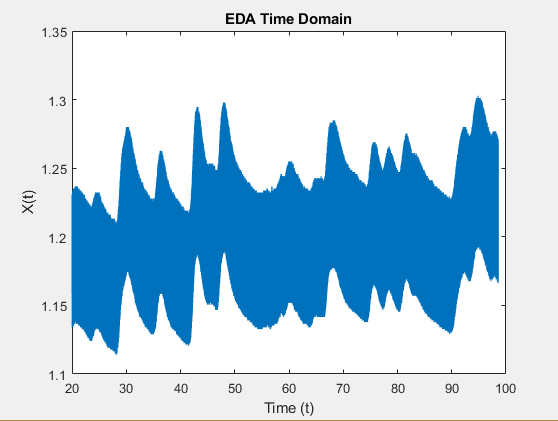
\includegraphics[width=0.9\textwidth]{images/rawEDA.png}
\caption{Raw data of an EDA measurement.}
\label{rawEDAImg}
\end{figure}

\begin{figure}[ht]
\centering
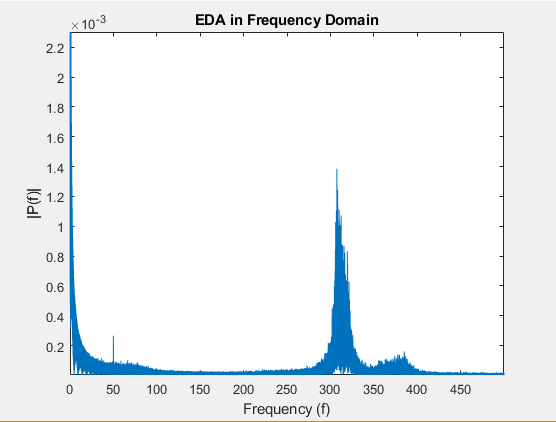
\includegraphics[width=0.9\textwidth]{images/fftEDA.png}
\caption{FFT of an EDA raw data set.}
\label{fftEDAImg}
\end{figure}

Once the general preprocessing of the data was finished we continued by applying specific filtering methods to each signal in regard to the FFT results.

\subsubsection{ECG Processing}
%-filter
Our main goal was to enhance the ECG signal for optimized feature extraction, particularly heart rate (HR) and heart rate variation (HRV). We therefore have tried two different approaches of filtering. The first method involved a Savitzky-Golay FIR smoothing filter that was part of an algorithm specifically designed for the BITalino device and recommended by the producing company. Savitzky-Golay filter are usually used on signals that have a large frequency span even without noise. Considering that, frequencies from 0.01Hz to 250Hz are contained in a typical ECG signal it seemed appropriate to use it \cite{tan2013digital}.
The second method was based on literature and the evaluation of the frequency analysis.
As the frequency analysis had shown a spike at 50 Hz, which was most likely caused by the power line interference, we applied a notch filter with a notch frequency f0 of 50Hz and a notch width of 0,1 Hz to eliminate the 50Hz hum from our signal.
In addition to this we had to remove muscle noise, which may occured at approximately 40Hz and removed the effects of a possible DC drift \cite{tan2013digital}.
After detrending, using the Matlab function \textit{detrend(X)} we used a Butterworth bandpass filter with a bandpass from 5 Hz to 26 Hz and filter order 4. This filter provided a magnitude response that is maximally flat in the passband and monotonic overall.  

\subsubsection{EDA Processing}

%-filter


%-substract baseline


\subsection{Feature Extraction}
%-time vector
% first step visual inspection of the signal


%- how many subjects did participate?\\
%- which tasks did the patients fullfill? (cross the bridge etc.)\\
%- duration of the experiment\\
%
%- description of the virtual environment, the procedure (baseline measurement,VRET in detail)\\ 
%- pictures that show the VE in it's starting state as well as it's therapy state (descended floor)\\
%- description of how the VR is controlled by the user(which parameters can be influenced)
%
%
%-ECG processing frequency domain methods PSD (in task force , reason which method to pick)

